\documentclass{standalone}
\usepackage{hsbcommon}
\begin{document}
    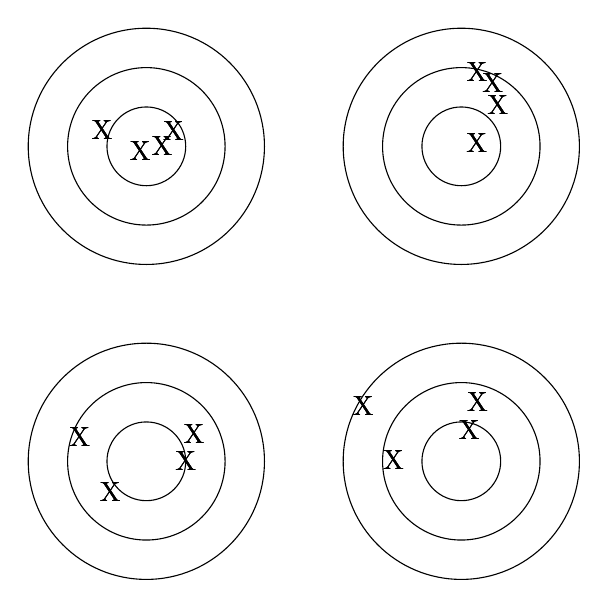
\begin{tikzpicture}
            \tikzset{pics/.cd,
              pic a/.style={code={
                  \node at (0:0.2) {X};
                  \node at (30:0.4) {X};
                  \node at (220:0.1) {X};
                  \node at (160:0.6) {X};
              }},
              pic b/.style={code={
                  \node at (0:0.5) {X};
                  \node at (30:0.7) {X};
                  \node at (220:0.6) {X};
                  \node at (160:0.9) {X};
              }}
            }
            \foreach \ii in {0.5,1,1.5} {
            \draw (0,0) circle (\ii);
                \pic at (0,0) {pic a};
            }
            \foreach \ii in {0.5,1,1.5} {
            \draw (4,0) circle (\ii);
                \pic[rotate=90] at (4.4,0.6) {pic a};
            }
            \foreach \ii in {0.5,1,1.5} {
            \draw (0,-4) circle (\ii);
                \pic at (0,-4) {pic b};
            }
           \foreach \ii in {0.5,1,1.5} {
            \draw (4,-4) circle (\ii);
                \pic at (3.6,-3.6) {pic b};
            }
    \end{tikzpicture}

\end{document}
